\documentclass{beamer}
\usepackage{listings}
\usepackage{xcolor}

\usetheme{Madrid}
\usecolortheme{seahorse}
\definecolor{codegreen}{rgb}{0,0.6,0}
\definecolor{codegray}{rgb}{0.5,0.5,0.5}
\definecolor{codepurple}{rgb}{0.58,0,0.82}
\definecolor{backcolour}{rgb}{0.95,0.95,0.92}

% Define code listing style
\lstdefinestyle{mystyle}{
    backgroundcolor=\color{backcolour},   
    commentstyle=\color{codegreen},
    keywordstyle=\color{magenta},
    numberstyle=\tiny\color{codegray},
    stringstyle=\color{codepurple},
    basicstyle=\ttfamily\footnotesize,
    breakatwhitespace=false,         
    breaklines=true,                 
    captionpos=b,                    
    keepspaces=true,                 
    numbers=left,                    
    numbersep=5pt,                  
    showspaces=false,                
    showstringspaces=false,
    showtabs=false,                  
    tabsize=2
}
\lstset{
  basicstyle=\ttfamily\small,
  columns=fullflexible,
  keepspaces=true,
  frame=single,
  language=C,
  commentstyle=\color{green!50!black},
  keywordstyle=\color{blue},
  numbers=left,
  numberstyle=\tiny,
  stepnumber=1,
  numbersep=5pt,
}


% Title page information
\title{Selection And Merge Sort }
\author{Group:04}
\date{\today}

% Custom block environment
\newenvironment{customblock}[1]
  {\begin{block}{#1}\begin{flushleft}\ttfamily}
  {\end{flushleft}\end{block}}

\begin{document}

% Custom title page
\begin{frame}[plain]
  \titlepage
  \begin{figure}
    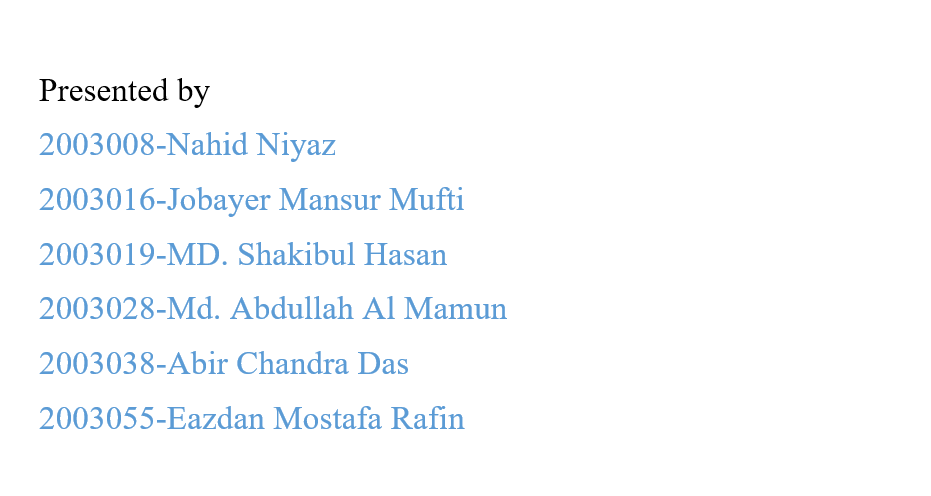
\includegraphics[width=0.5\textwidth]{graphics/Names1.png} % Replace "your_image_filename" with the actual filename of your image
  \end{figure}
\end{frame}



\title{Selection Sort}
\author{}
\date{}

% Custom color
\definecolor{myblue}{RGB}{30,80,120}



\begin{frame}
  \titlepage
\end{frame}


\begin{frame}{Key Points - Selection Sort}
  \begin{itemize}
    \item Selection Sort is a simple sorting algorithm.
    \item It works by finding the minimum or maximum element in the unsorted part of the array and placing it in the sorted part.
    \item In each pass, one element is sorted. For $n$ elements, $n-1$ passes are required.
    \item The algorithm starts by setting the first element as the minimum.
    \item It then compares the minimum with the second element. If the second element is smaller, it assigns the second element as the new minimum.
    \item This process is repeated for each element in the unsorted part of the array until the last element is reached.
    \item After each pass, the minimum is placed at the front of the unsorted list.
    \item Indexing starts from the first unsorted element after each pass.
    \item The algorithm can sort the array in ascending or descending order, depending on whether it finds the minimum or maximum element in each iteration.
    \item Not suitable for large datasets due to its average and worst-case complexities of $O(n^2)$.
  \end{itemize}
\end{frame}

\begin{frame}[fragile]{Selection Sort Algorithm}
  \begin{lstlisting}[language=C++]
    void selectionSort(int arr[], int n) {
        for (int i = 0; i < n-1; i++) {
            int minIndex = i;
            for (int j = i+1; j < n; j++) {
                if (arr[j] < arr[minIndex]) {
                    minIndex = j;
                }
            }
            // Swap the found minimum element with the first element
            int temp = arr[minIndex];
            arr[minIndex] = arr[i];
            arr[i] = temp;
        }
    }
    \end{lstlisting}
\end{frame}

\begin{frame}{Selection Sort Step-by-Step}
  \begin{customblock}{Selection Sort Steps}
    \begin{itemize}
      \item Start with the first element as the minimum.
      \item Compare the minimum with the second element. If the second element is smaller, update the minimum.
      \item Repeat the process for each element in the unsorted part of the array until the last element is reached.
      \item After each pass, place the minimum at the front of the unsorted list.
      \item Move to the next unsorted element and repeat the process until the entire array is sorted.
    \end{itemize}
  \end{customblock}
\end{frame}


\begin{frame}{Selection Sort Visualization}
  \begin{figure}
    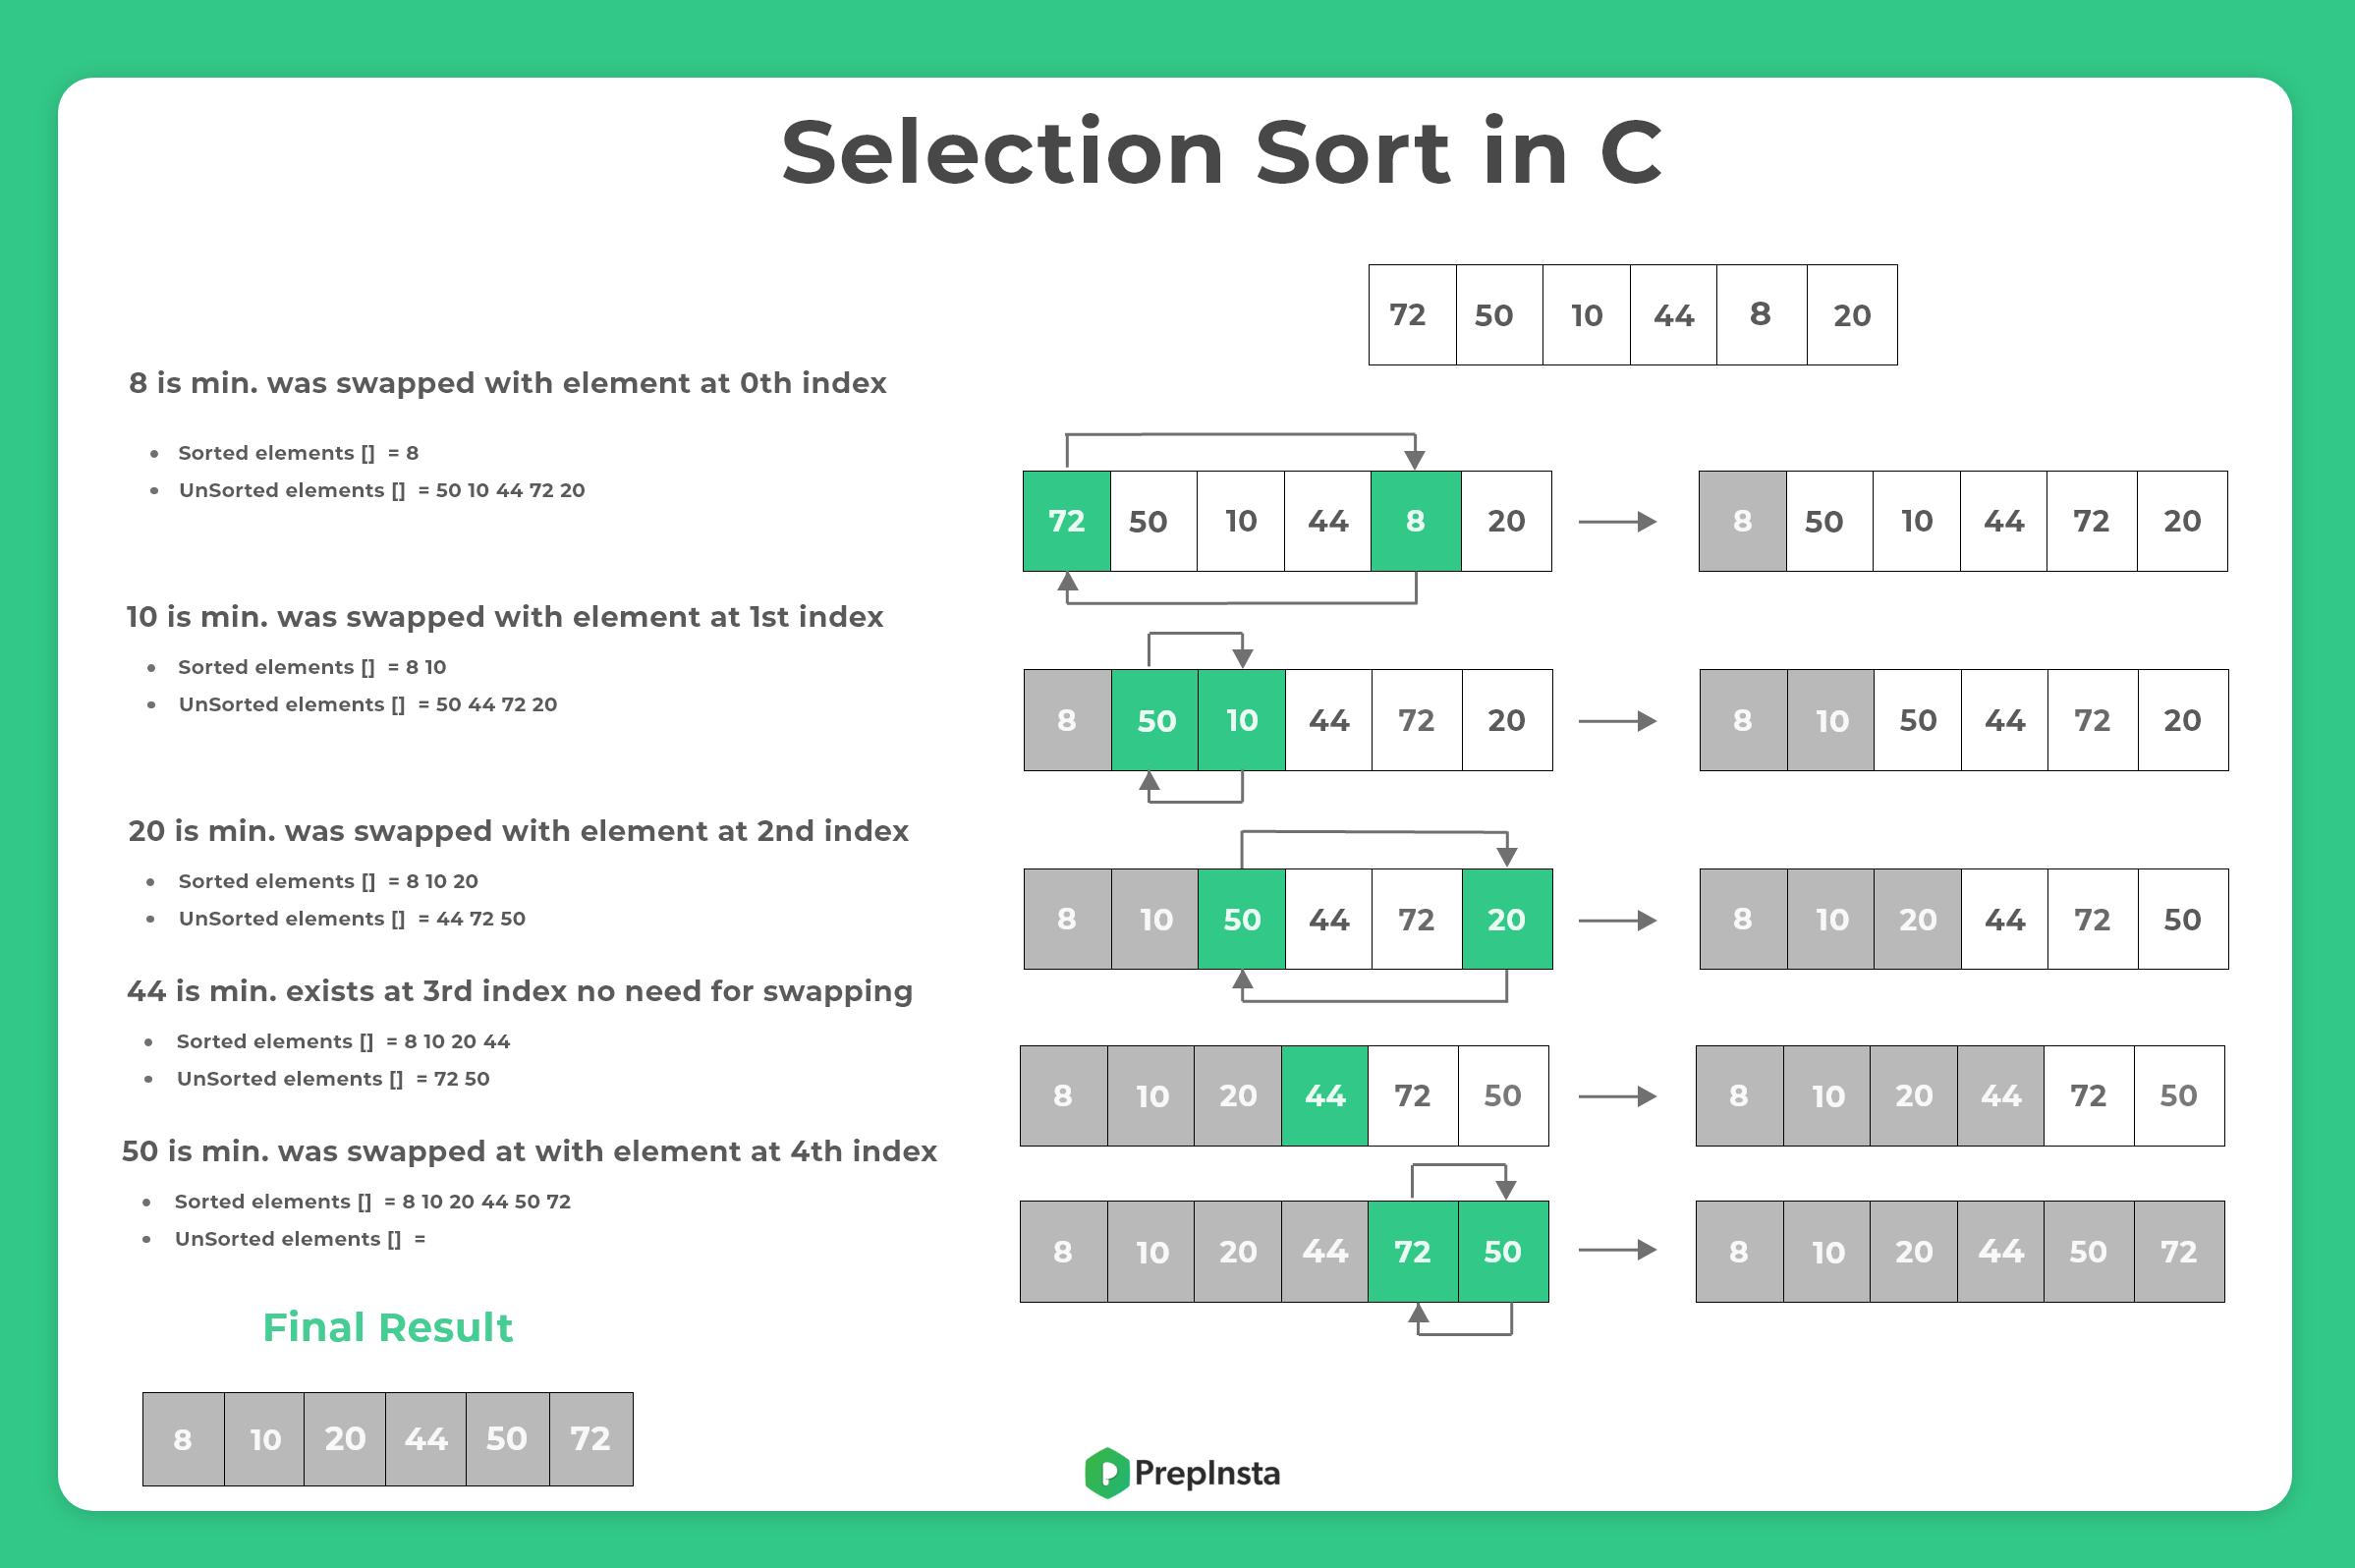
\includegraphics[width=0.8\textwidth]{graphics/Selection-sort1.png}
    \caption{Selection Sort Visualization}
  \end{figure}
\end{frame}

\begin{frame}{Time Complexity of Selection Sort}
  \begin{itemize}
    \item Selection Sort has a time complexity of $O(n^2)$ in both the average and worst cases.
    \item For each element in the array, it needs to traverse the remaining unsorted part to find the minimum or maximum element.
    \item The nested loop structure results in quadratic time complexity.
    \item Inefficient for large datasets as the number of comparisons and swaps grows quadratically with the size of the input.
    \item Despite its simplicity, it's not suitable for large datasets compared to more efficient sorting algorithms.
  \end{itemize}
\end{frame}

\begin{frame}{Application of Selection Sort}
  \begin{itemize}
    \item \textbf{\color{blue}Small Datasets:}
          \begin{itemize}
            \item Selection Sort can be suitable for sorting small datasets where its simplicity may outweigh its relatively higher time complexity.
          \end{itemize}
    \item \textbf{\color{blue}Educational Purposes:}
          \begin{itemize}
            \item It is often used in educational settings to introduce the concept of sorting algorithms due to its straightforward logic.
          \end{itemize}
    \item \textbf{\color{blue}Memory Usage:}
          \begin{itemize}
            \item Selection Sort is an in-place sorting algorithm, meaning it doesn't require additional memory space, making it useful in situations with limited memory.
          \end{itemize}
    \item \textbf{\color{blue}Stable Sorting:}
          \begin{itemize}
            \item While not stable by default, modifications can be made to Selection Sort to make it stable (maintaining the relative order of equal elements).
          \end{itemize}
  \end{itemize}
\end{frame}

\title{Merge Sort}
\author{}
\date{}

% Custom color
\definecolor{myblue}{RGB}{30,80,120}



\begin{frame}
  \titlepage
\end{frame}



\begin{frame}{Introduction to Merge Sort}
  \begin{block}{Key Points}
    \begin{itemize}
      \item Merge Sort is a popular sorting algorithm.
      \item It follows the \textbf{divide-and-conquer} paradigm.
            \begin{itemize}
              \item \textbf{Divide :} The unsorted list is recursively divided into smaller sublists until each sublist contains only one element
              \item \textbf{conquer :} Once the list is divided into individual elements (each considered a sorted sublist of size 1), the algorithm starts merging these sublists in a way that builds up a sorted order. This is the "conquer" step, where the individual sorted sublists are merged to produce larger sorted sublists.
            \end{itemize}
      \item Efficient for large datasets.
    \end{itemize}
  \end{block}
\end{frame}

\begin{frame}[fragile]{Merge Sort Algorithm}

  \begin{enumerate}
    \item Divide the unsorted list into \(n\) sublists.
          %    \item Repeatedly merge sublists.
  \end{enumerate}

  \begin{lstlisting}[caption={Merge Sort in C++}, label=mergeSortCode]
void merge_sort(int ax[], int lb, int ub) {
    if (lb < ub) {
        int mid = (lb + ub) / 2;
        merge_sort(ax, lb, mid);
        merge_sort(ax, mid + 1, ub);
        merge(ax, lb, mid, ub);
    }
}
    \end{lstlisting}

\end{frame}
\begin{frame}[fragile, shrink=10]{Merge Sort Algorithm}

  \begin{enumerate}
    \item Repeatedly merge sublists.
  \end{enumerate}

  \begin{lstlisting}[caption={Merge Sort in C++}, label=mergeSortCode]
void merge(int ax[], int lb, int mid, int ub) {
  int i, j, k;
  i = lb;
  j = mid + 1;
  k = lb;
  int bx[n];
  while (i <= mid && j <= ub) {
      if (ax[i] <= ax[j]) {
          bx[k] = ax[i];
          i++;
          k++;
      } else {
          bx[k] = ax[j];
          j++;
          k++;
      }
  }
  if (i > mid) {
      while (j <= ub) {
          bx[k] = ax[j];
          j++;
          k++;
      }
  } else {
      while (i <= mid) {
          bx[k] = ax[i];
          i++;
          k++;
      }
  }
  for (int k = lb; k <= ub; k++) {
      ax[k] = bx[k];
  }
}
  \end{lstlisting}

\end{frame}
\begin{frame}{Merge Sort Example}
  \begin{figure}
    \centering
    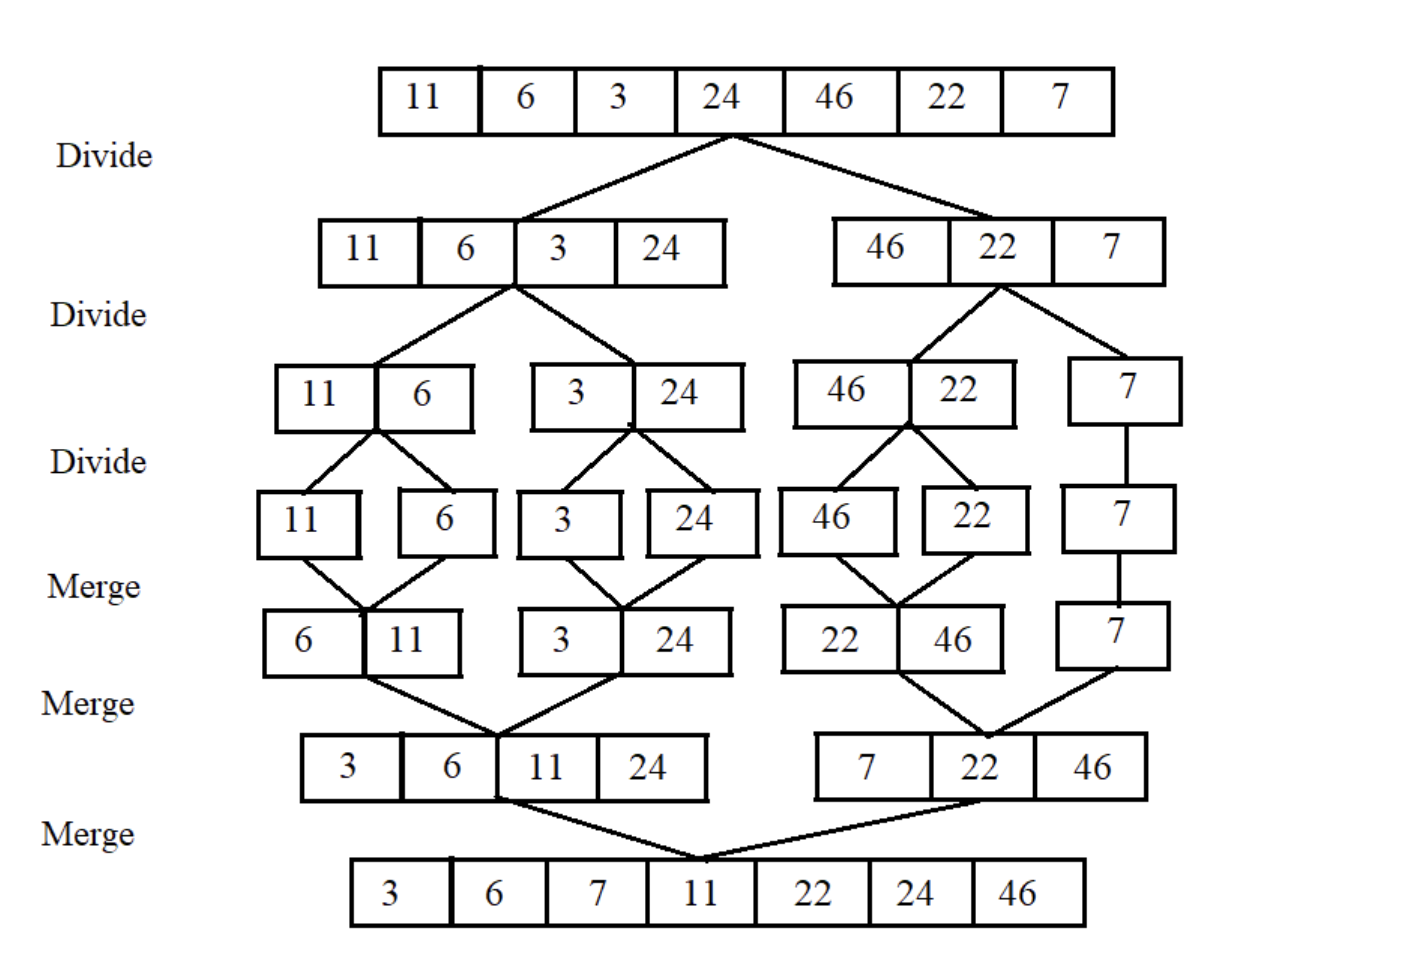
\includegraphics[width=0.8\textwidth]{graphics/merge.png}
    \caption{Illustration of the Merge Sort Algorithm}
  \end{figure}
\end{frame}




\begin{frame}{Time Complexity of Merge Sort}
  \begin{block}{Complexity Analysis}
    \begin{figure}
      \centering
      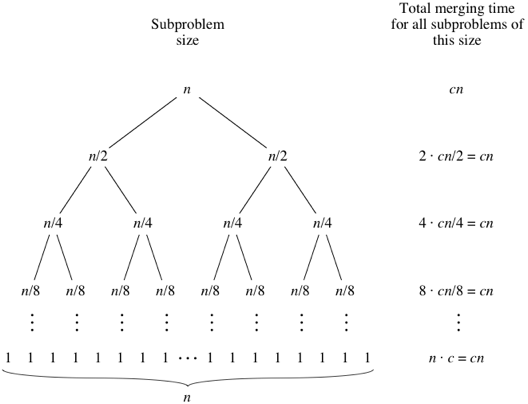
\includegraphics[width=0.8\textwidth]{graphics/mergetree.png}
      % \caption{Illustration of the Merge Sort Algorithm}
    \end{figure}
    % \begin{itemize}
    %   \item Merge Sort: \(O(n \log n)\)
    %   \item Efficient for large datasets.
    % \end{itemize}
  \end{block}
\end{frame}
\begin{frame}{Time Complexity of Merge Sort}
  \begin{block}{Complexity Analysis}
    \begin{figure}
      \centering
      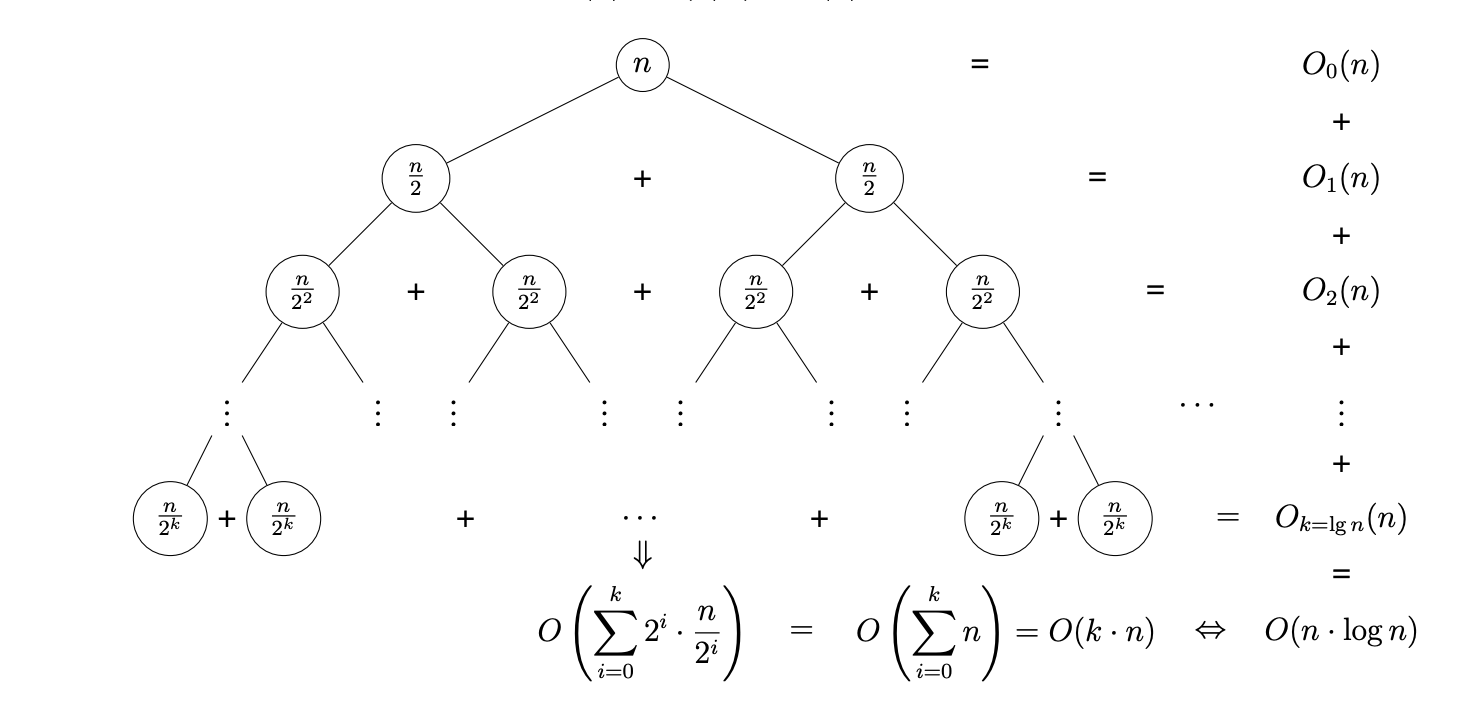
\includegraphics[width=1\textwidth]{graphics/mergetree_2.png}
      % \caption{Illustration of the Merge Sort Algorithm}
    \end{figure}

  \end{block}
\end{frame}
\begin{frame}{Time Complexity of Merge Sort}
  \begin{block}{Complexity Analysis}
    \begin{itemize}
      \item The divide step takes constant time.\(O(1)\)
      \item Total Merging Time = \(l*c*n\)
            \begin{itemize}
              \item Here, \(l=O(n \log n)+1\)
              \item So,Total Merging Time will Be =\(O(n \log n)\)
            \end{itemize}
      \item Efficient for large datasets.
    \end{itemize}
  \end{block}
\end{frame}
\begin{frame}{Merge Sort Time Complexity - Recursive Function}
  \begin{block}{Time Complexity Recurrence Relation}
    The time complexity of Merge Sort is often expressed using the recurrence relation:
    \[ T(n) = 2T\left(\frac{n}{2}\right) + O(n) \]
  \end{block}
  \begin{block}{Time Complexity Breakdown}
    \begin{itemize}
      \item \( T(n) \): Time complexity for an input of size \( n \).
      \item \( 2T\left(\frac{n}{2}\right) \): Time complexity for dividing the array into two halves and recursively sorting each half.
      \item \( O(n) \): Time complexity for merging the two sorted segments.
    \end{itemize}

  \end{block}

  \begin{block}{Master Theorem Analysis}
    Applying the Master Theorem to the recurrence relation yields a time complexity of \(O(n \log n)\).
  \end{block}

\end{frame}

\begin{frame}{Merge Sort Time Complexity - Recursive Function}
  \begin{figure}
    \centering
    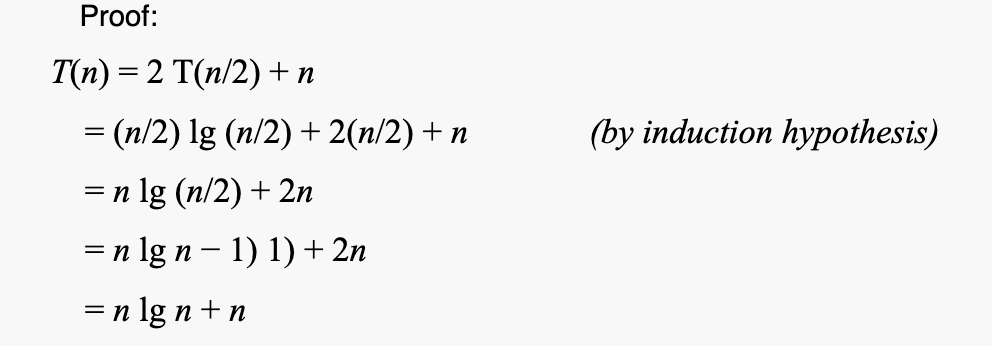
\includegraphics[width=1\textwidth]{graphics/time.png}
    % \caption{Illustration of the Merge Sort Algorithm}
  \end{figure}

\end{frame}
\begin{frame}{Space Complexity of Merge Sort}
  \begin{block}{Memory Usage}
    Merge sort has a space complexity of \(O(n)\) due to the need for additional memory to store temporary arrays during the merging process.
  \end{block}

  \begin{block}{Explanation}
    \begin{itemize}
      \item Merge sort divides the array into halves recursively, requiring additional memory for each recursive call.
      \item The merging step involves copying elements to a temporary array, adding to the overall space complexity.
      \item The total space complexity is \(O(n)\) as the maximum depth of the recursion is \(\log n\) and at each level, \(n\) elements are stored.
    \end{itemize}
  \end{block}

  \begin{block}{Summery of Space Complexity}
    While merge sort has an optimal time complexity, its space complexity may be a consideration for large datasets with limited memory.
  \end{block}
\end{frame}

\begin{frame}{Applications For Merge Sort}
  % \begin{alertblock}{Key Takeaways}
  %   \begin{itemize}
  %     \item Merge Sort is reliable and efficient.
  %     \item Guarantees \(O(n \log n)\) time complexity.
  %     \item Widely used for its performance.
  %   \end{itemize}
  % \end{alertblock}

  \begin{exampleblock}{Real-Life Applications}
    \begin{itemize}
      \item \textbf{External Sorting:} Used in scenarios with large datasets that don't fit in main memory.
      \item \textbf{Database Management:} Efficient sorting in database systems.
      \item \textbf{Network Routing:} Sorting routes to optimize network communication.
      \item \textbf{Parallel Processing:} Suitable for parallel computing environments.
      \item \textbf{File Merging:} Merging sorted files efficiently.
      \item \textbf{Flight Scheduling:} Organizing flight information based on criteria.
      \item \textbf{Inversion Counting:} Useful in data analysis, statistics, and optimization.
      \item \textbf{External Memory Algorithms:} Widely used in algorithms for large external datasets.
    \end{itemize}
  \end{exampleblock}
\end{frame}
\begin{frame}{Merge Sort vs. Selection Sort}
  \begin{columns}
    \column{0.4\textwidth}
    \begin{block}{Merge Sort}
      \begin{itemize}
        \item Uses a divide and conquer strategy.
        \item Guaranteed time complexity: \(O(n \log n)\).
        \item Efficient for large datasets.
        \item Stable sorting algorithm.
      \end{itemize}
    \end{block}

    \column{0.4\textwidth}
    \begin{block}{Selection Sort}
      \begin{itemize}
        \item Simple and intuitive.
        \item Guaranteed time complexity: \(O(n^2)\).
        \item Inefficient for large datasets.
        \item In-place sorting algorithm.
      \end{itemize}
    \end{block}
  \end{columns}

  \vspace{1em}

  \begin{figure}
    \centering
    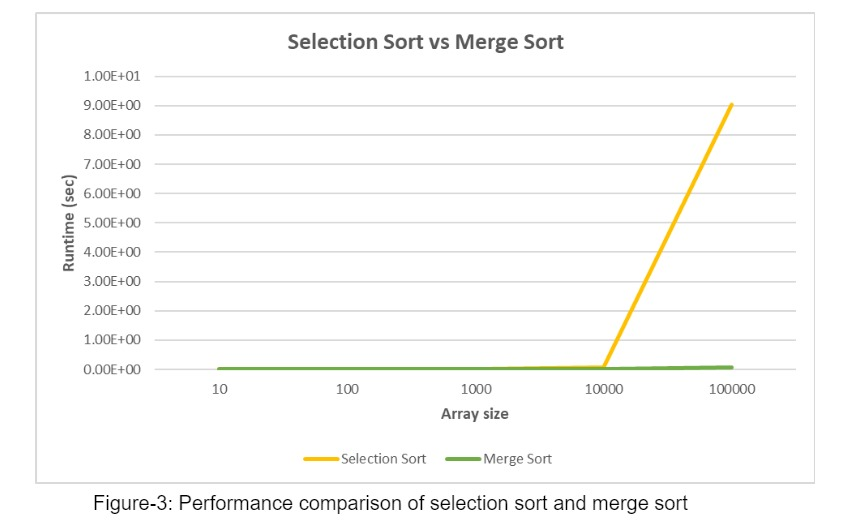
\includegraphics[width=0.5\textwidth]{graphics/sm.jpeg}
    \caption{Comparison of Merge Sort and Selection Sort}
  \end{figure}
\end{frame}



\end{document}